\section{Base\-Activity Class Reference}
\label{classBaseActivity}\index{BaseActivity@{BaseActivity}}
Inheritance diagram for Base\-Activity:\begin{figure}[H]
\begin{center}
\leavevmode
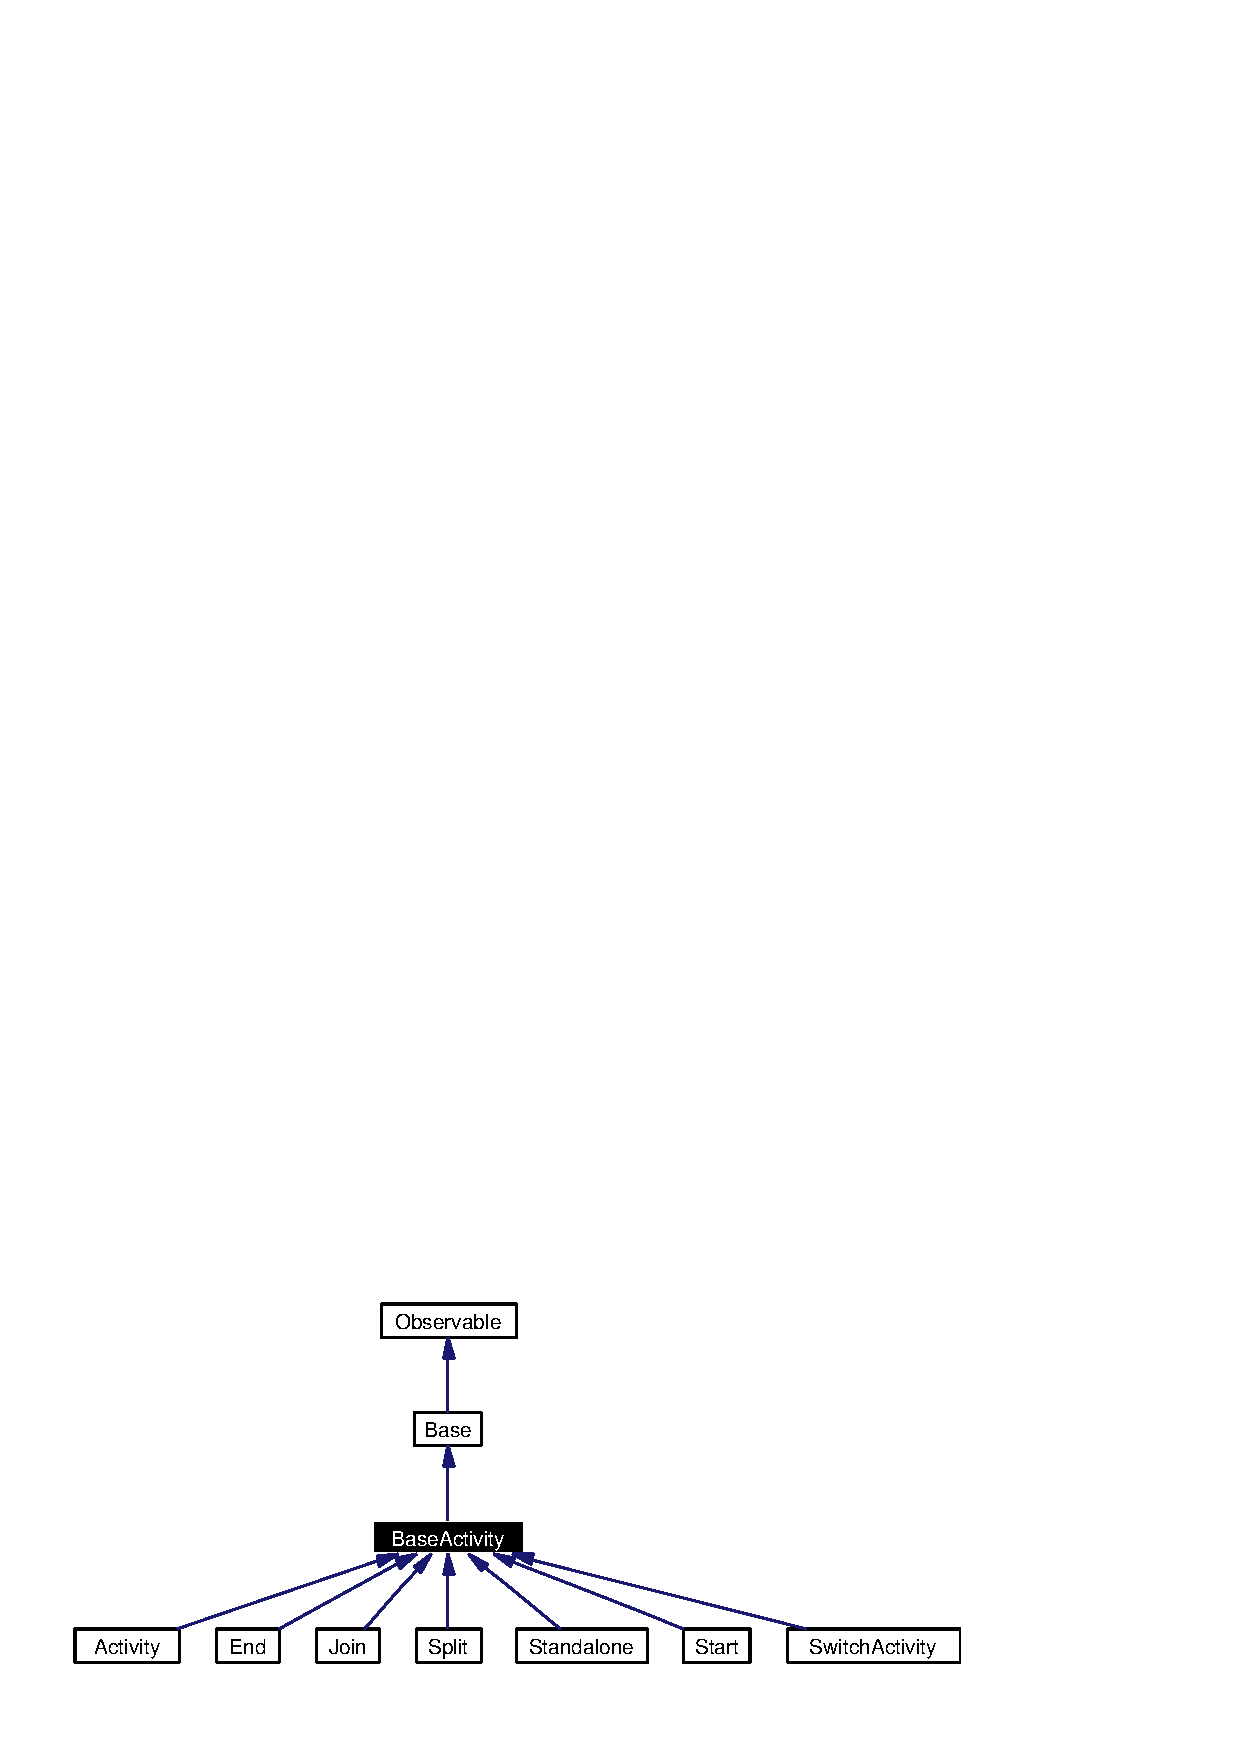
\includegraphics[width=230pt]{classBaseActivity__inherit__graph}
\end{center}
\end{figure}
Collaboration diagram for Base\-Activity:\begin{figure}[H]
\begin{center}
\leavevmode
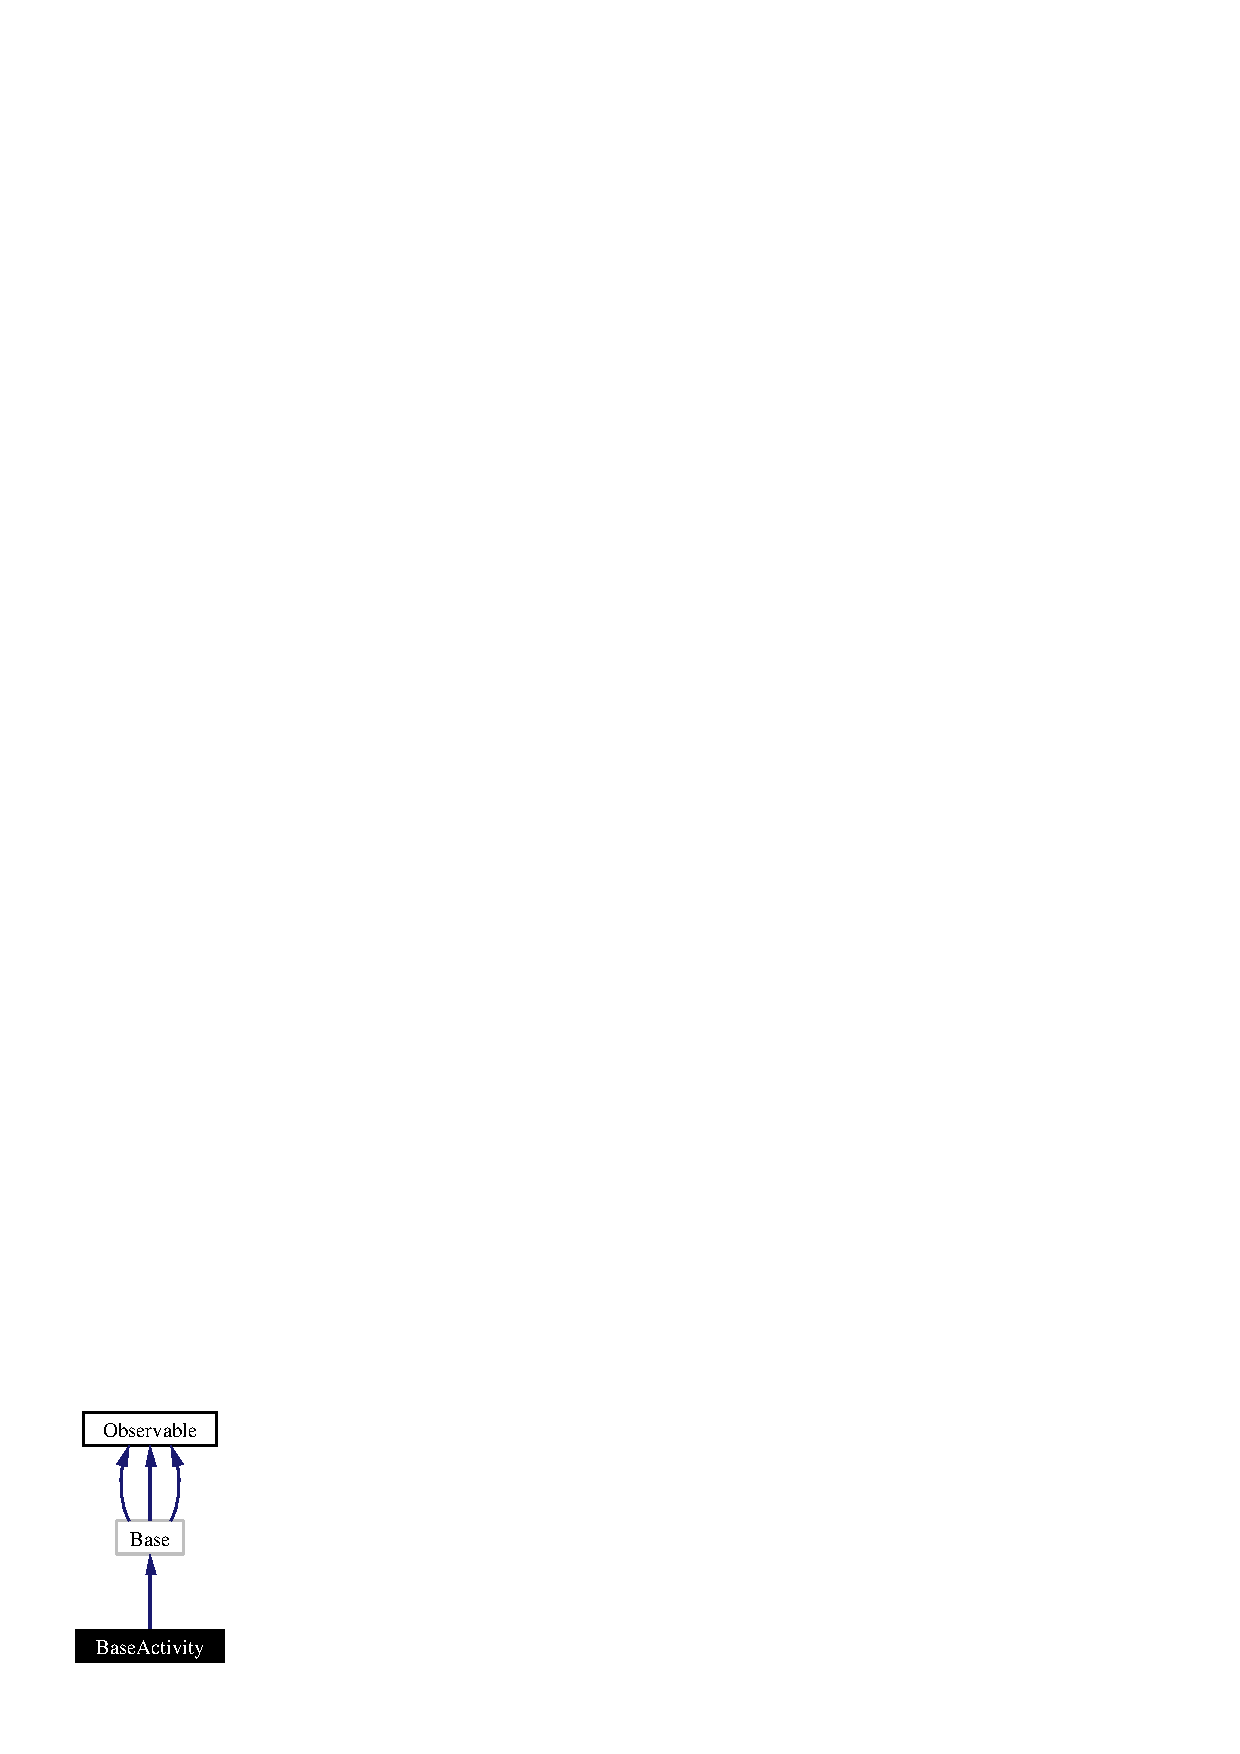
\includegraphics[width=54pt]{classBaseActivity__coll__graph}
\end{center}
\end{figure}
\subsection*{Public Member Functions}
\begin{CompactItemize}
\item 
{\bf get\-Activity} (\$activity\-Id)
\end{CompactItemize}
\subsection*{Public Attributes}
\begin{CompactItemize}
\item 
\index{name@{name}!BaseActivity@{BaseActivity}}\index{BaseActivity@{BaseActivity}!name@{name}}
{\bf name}\label{classBaseActivity_m0}

\item 
\index{normalized_name@{normalized\_\-name}!BaseActivity@{BaseActivity}}\index{BaseActivity@{BaseActivity}!normalized_name@{normalized\_\-name}}
{\bf normalized\_\-name}\label{classBaseActivity_m1}

\item 
\index{description@{description}!BaseActivity@{BaseActivity}}\index{BaseActivity@{BaseActivity}!description@{description}}
{\bf description}\label{classBaseActivity_m2}

\item 
\index{isInteractive@{isInteractive}!BaseActivity@{BaseActivity}}\index{BaseActivity@{BaseActivity}!isInteractive@{isInteractive}}
{\bf is\-Interactive}\label{classBaseActivity_m3}

\item 
\index{isAutoRouted@{isAutoRouted}!BaseActivity@{BaseActivity}}\index{BaseActivity@{BaseActivity}!isAutoRouted@{isAutoRouted}}
{\bf is\-Auto\-Routed}\label{classBaseActivity_m4}

\item 
\index{roles@{roles}!BaseActivity@{BaseActivity}}\index{BaseActivity@{BaseActivity}!roles@{roles}}
{\bf roles} = Array()\label{classBaseActivity_m5}

\item 
\index{outbound@{outbound}!BaseActivity@{BaseActivity}}\index{BaseActivity@{BaseActivity}!outbound@{outbound}}
{\bf outbound} = Array()\label{classBaseActivity_m6}

\item 
\index{inbound@{inbound}!BaseActivity@{BaseActivity}}\index{BaseActivity@{BaseActivity}!inbound@{inbound}}
{\bf inbound} = Array()\label{classBaseActivity_m7}

\end{CompactItemize}


\subsection{Detailed Description}
This class represents activities, and must be derived for each activity type supported in the system. Derived activities extending this class can be found in the activities subfolder. This class is observable. 



Definition at line 10 of file Base\-Activity.php.

\subsection{Member Function Documentation}
\index{BaseActivity@{Base\-Activity}!getActivity@{getActivity}}
\index{getActivity@{getActivity}!BaseActivity@{Base\-Activity}}
\subsubsection{\setlength{\rightskip}{0pt plus 5cm}Base\-Activity::get\-Activity (\$ {\em activity\-Id})}\label{classBaseActivity_a0}


Factory method returning an activity of the desired type loading the information from the database. 

Definition at line 24 of file Base\-Activity.php.

The documentation for this class was generated from the following file:\begin{CompactItemize}
\item 
Base\-Activity.php\end{CompactItemize}
